% Solution_Template.tex
\documentclass[11pt,a4paper]{article}
\usepackage[utf8]{inputenc}
\usepackage[T1]{fontenc}
\usepackage[ngerman, english]{babel} % remove ngerman if you prefer English only
\usepackage{geometry}
\usepackage{fancyhdr}
\usepackage{hyperref}
\usepackage[utf8]{inputenc}
\usepackage{amsmath,amssymb,amsthm}
\usepackage{enumitem,setspace}
\usepackage[usenames,dvipsnames,table]{xcolor}
\usepackage{graphicx}
\DeclareGraphicsExtensions{.pdf,.png,.eps,.jpg}
\usepackage{algorithm2e}
\usepackage{float}

% --- math operators ---
\usepackage{mathtools}
\DeclarePairedDelimiter\set{\{}{\}} % use $\set{1, 2, 3}$
\DeclarePairedDelimiter\abs{\lvert}{\rvert}
\DeclarePairedDelimiter\norm{\lVert}{\rVert}
\DeclarePairedDelimiter\ceils{\lceil}{\rceil}
\DeclarePairedDelimiter\floor{\lfloor}{\rfloor}
\def\then{\ensuremath{\Rightarrow}} % =>
\def\iff{\ensuremath{\Leftrightarrow}} % if and only if <=>
\def\to{\ensuremath{\rightarrow}} % ->
\def\ot{\ensuremath{\leftarrow}} % ->
\def\Oh{\ensuremath{\mathcal{O}}} % big O like $\Oh(n)$
% ---
\DeclareMathOperator{\preorder}{preorder}
\DeclareMathOperator{\postorder}{postorder}
\DeclareMathOperator{\depth}{depth}

\geometry{margin=25mm}
\pagestyle{fancy}
\fancyhf{}
\renewcommand{\headrulewidth}{0.4pt}
\lhead{\textbf{Name:} \studentname}
\rhead{\textbf{Matr.-Nr.:} \studentnumber}
\cfoot{\thepage}

% User info - edit these
\newcommand{\studentname}{Matthias Janßen}
\newcommand{\studentnumber}{1871808}
\newcommand{\course}{Übersetzung und Analyse von Programmen}
\newcommand{\institute}{Universität Trier}

\title{\course}
\author{\studentname\\Matrikelnummer: \studentnumber\\\institute}
\date{\today}

\begin{document}

\maketitle

\begin{center}
    \textbf{Abgabe:} Assignment / Sheet \\
    \vspace{4mm}
    \textbf{Betreuer:} Supervisor Name
\end{center}

\bigskip

\section*{Aufgaben}
% Start writing your solutions here.

\section{Aufgabe 1}
	a) Zeigen Sie, dass $L$ eine reguläre Sprache ist.\\
Die Sprache $L$ besteht aus allen Wörtern der Länge $5$ über dem Alphabet $\Sigma = \{a, b\}$, wobei das zweite und das vierte Zeichen gleich sind ($x_2 = x_4$) und das dritte und das fünfte Zeichen verschieden sind ($x_3 \neq x_5$).\\

Da $L$ nur Wörter der Länge $5$ betrachtet, ist $L$ eine endliche Sprache (es gibt nur $2^5 = 32$ mögliche Wörter). Jede endliche Sprache ist regulär, da man für jedes Wort einen eigenen Zweig im Automaten bauen kann.\\

Alternativ kann man $L$ auch als regulären Ausdruck angeben:
\[
L = \{ x_1 x_2 x_3 x_4 x_5 \in \Sigma^5 \mid x_2 = x_4 \wedge x_3 \neq x_5 \}
\]
Das ist eine endliche Vereinigung von Wörtern, also regulär.

	\smallskip b) Zeigen Sie, dass $\overline{L} := \Sigma^* \setminus L$ eine reguläre Sprache ist.\\
Die Klasse der regulären Sprachen ist unter Komplement abgeschlossen. Da $L$ regulär ist, ist auch das Komplement $\overline{L}$ regulär.\\

Alternativ: $\Sigma^*$ ist regulär, $L$ ist regulär $\Rightarrow \overline{L} = \Sigma^* \setminus L$ ist regulär.

\section{Aufgabe 2}
\centering
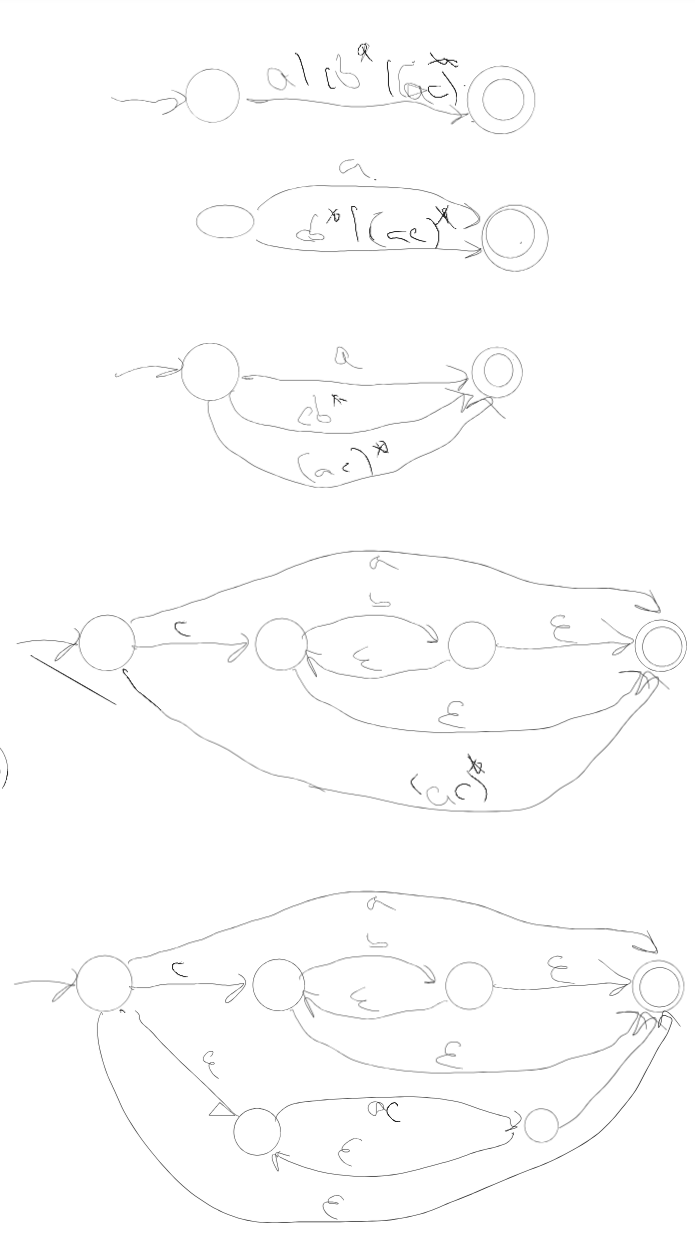
\includegraphics[width=0.6\linewidth]{nea.png} % use option [width=\linewidth] to change size to linewidth (or 0.6\linewidth for example)


%\centering
%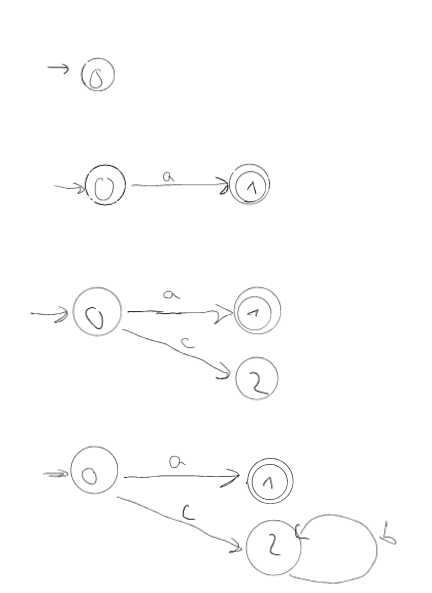
\includegraphics[width=0.6\linewidth]{nea1.png} % use option [width=\linewidth] to change size to linewidth (or 0.6\linewidth for example)

%\centering
%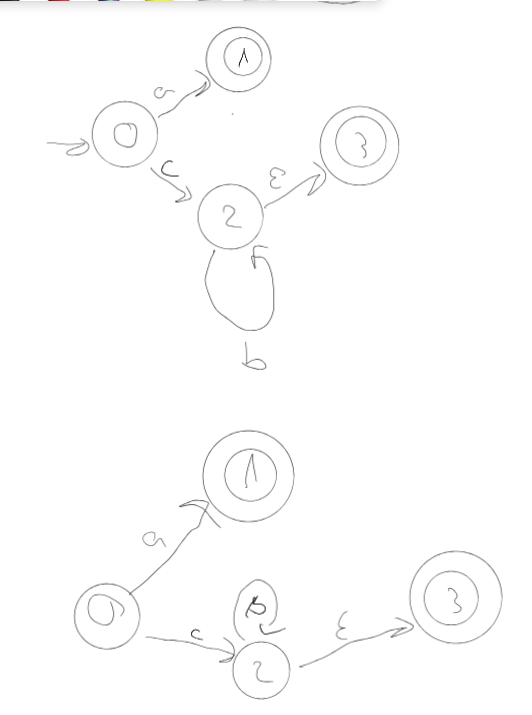
\includegraphics[width=0.6\linewidth]{nea2.png} % use option [width=\linewidth] to change size to linewidth (or 0.6\linewidth for example)

%\centering
%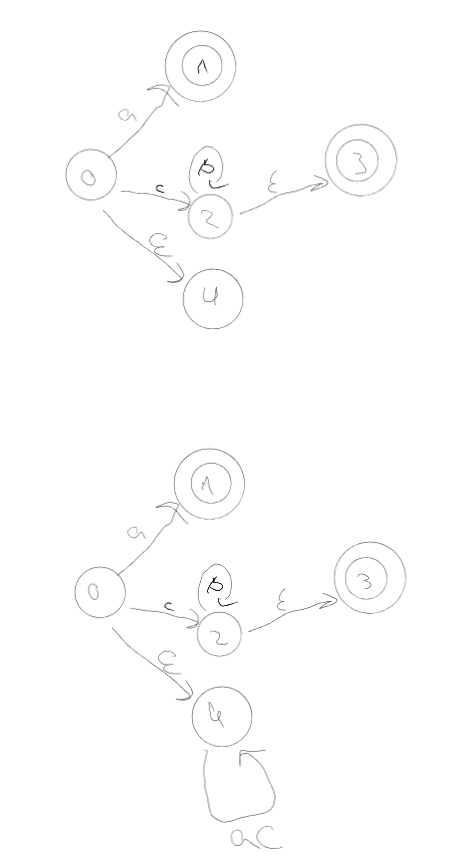
\includegraphics[width=0.6\linewidth]{nea3.png} % use option [width=\linewidth] to change size to linewidth (or 0.6\linewidth for example)

%\centering
%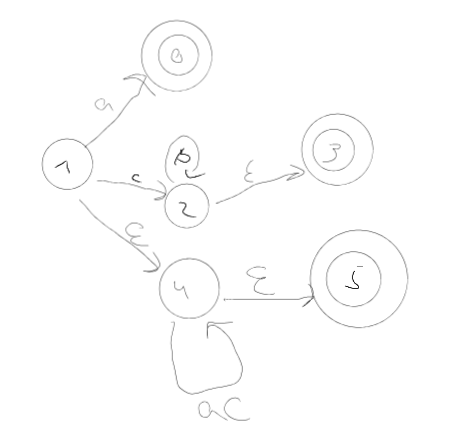
\includegraphics[width=0.6\linewidth]{nea4.png} % use option [width=\linewidth] to change size to linewidth (or 0.6\linewidth for example)

\bigskip
\section{Aufgabe 3}

\centering
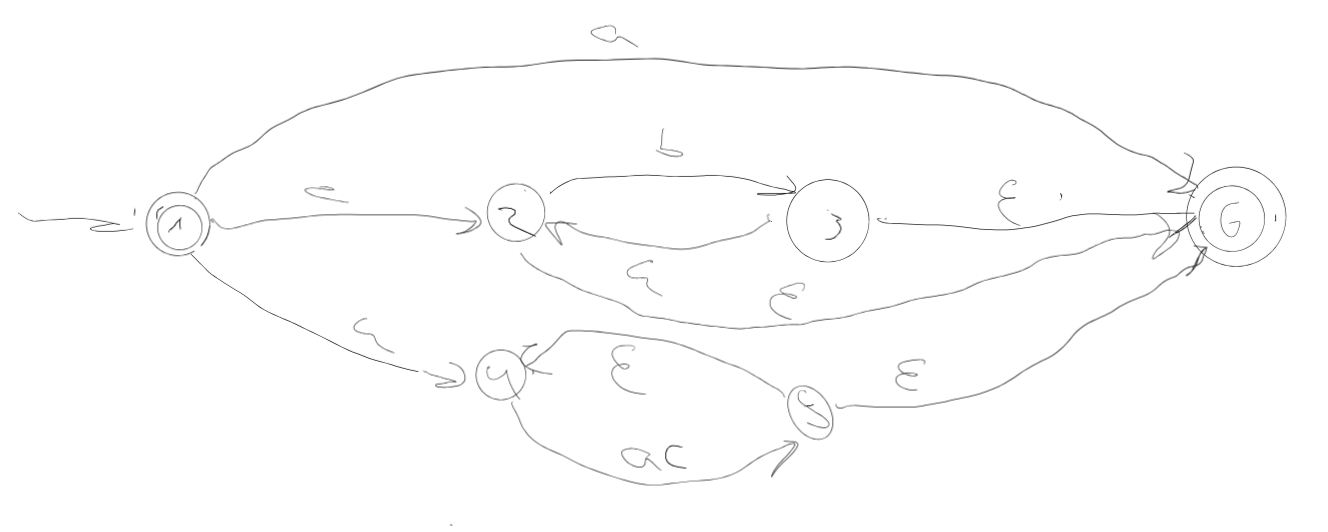
\includegraphics[width=0.6\linewidth]{dea1.png} % use option [width=\linewidth] to change size to linewidth (or 0.6\linewidth for example)

\centering
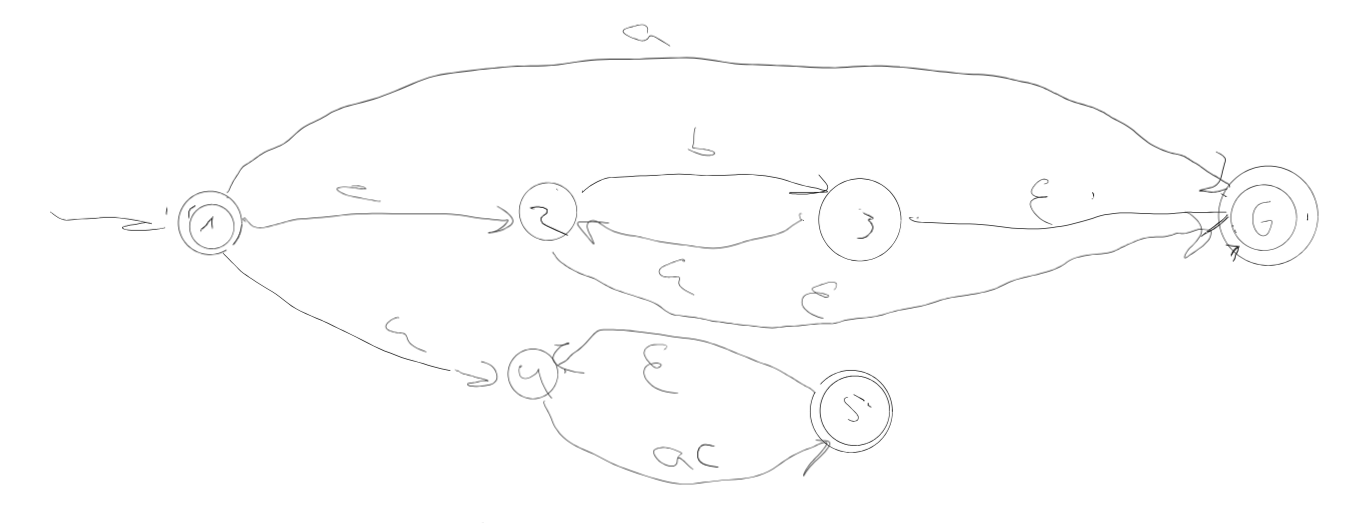
\includegraphics[width=0.6\linewidth]{dea2.png} % use option [width=\linewidth] to change size to linewidth (or 0.6\linewidth for example)


\centering
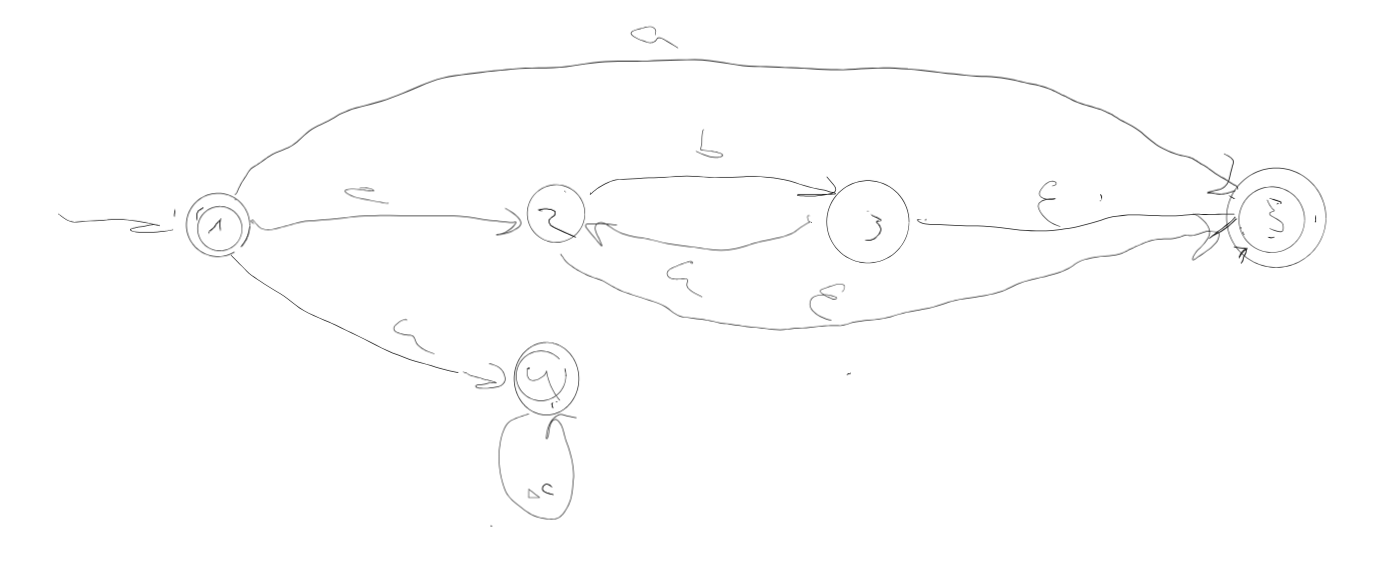
\includegraphics[width=0.6\linewidth]{dea3.png} % use option [width=\linewidth] to change size to linewidth (or 0.6\linewidth for example)

\centering
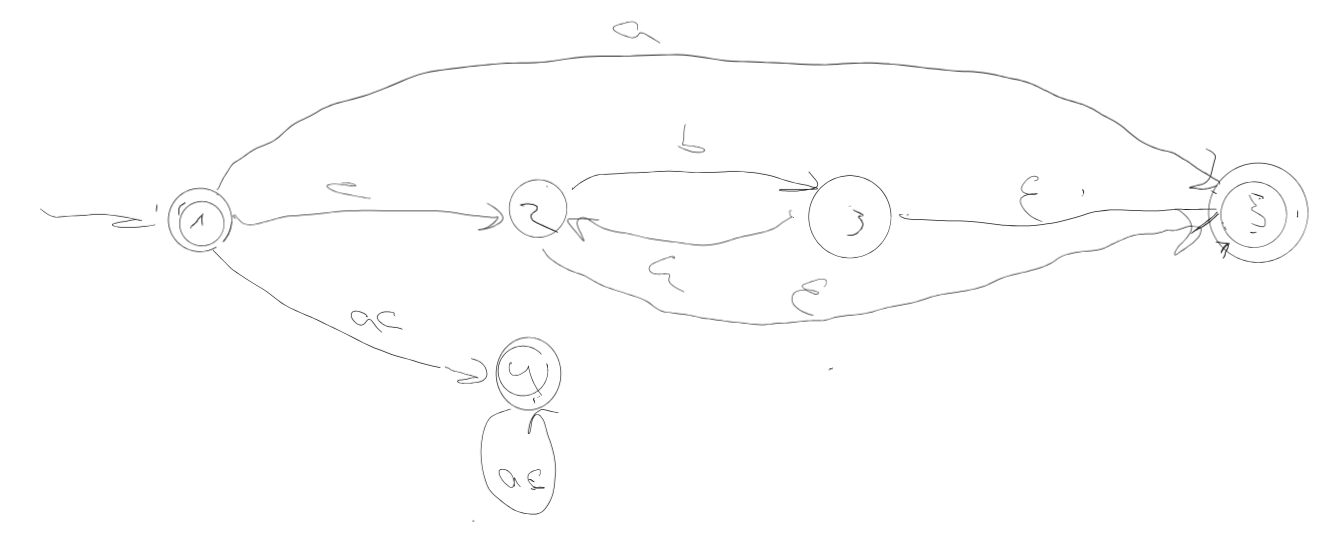
\includegraphics[width=0.6\linewidth]{dea4.png} % use option [width=\linewidth] to change size to linewidth (or 0.6\linewidth for example)

\centering
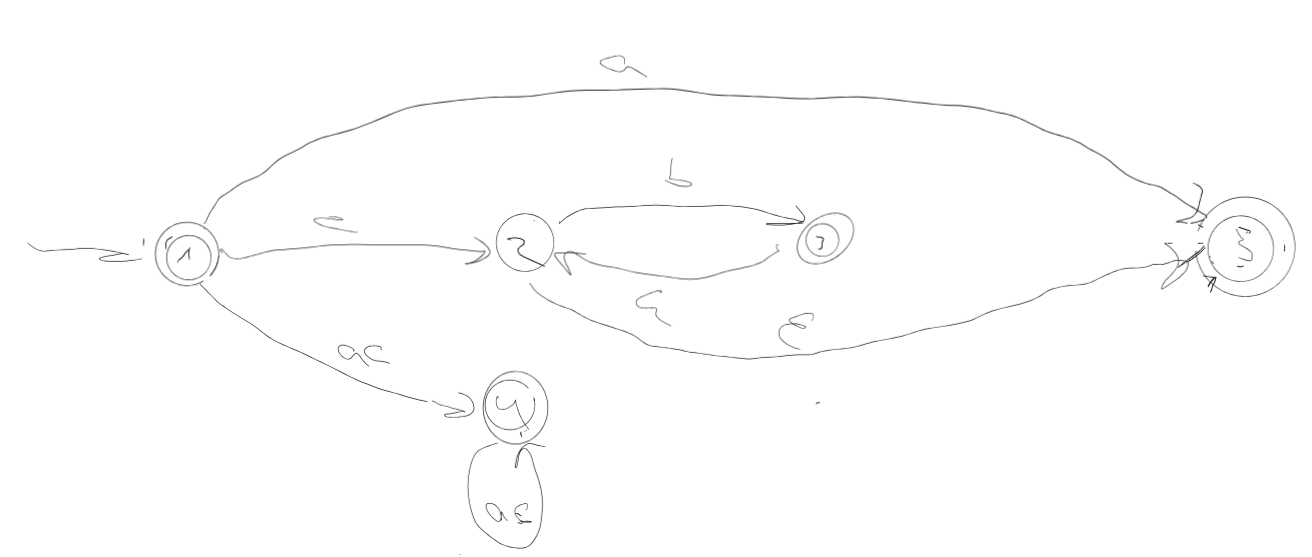
\includegraphics[width=0.6\linewidth]{dea5.png} % use option [width=\linewidth] to change size to linewidth (or 0.6\linewidth for example)

\centering
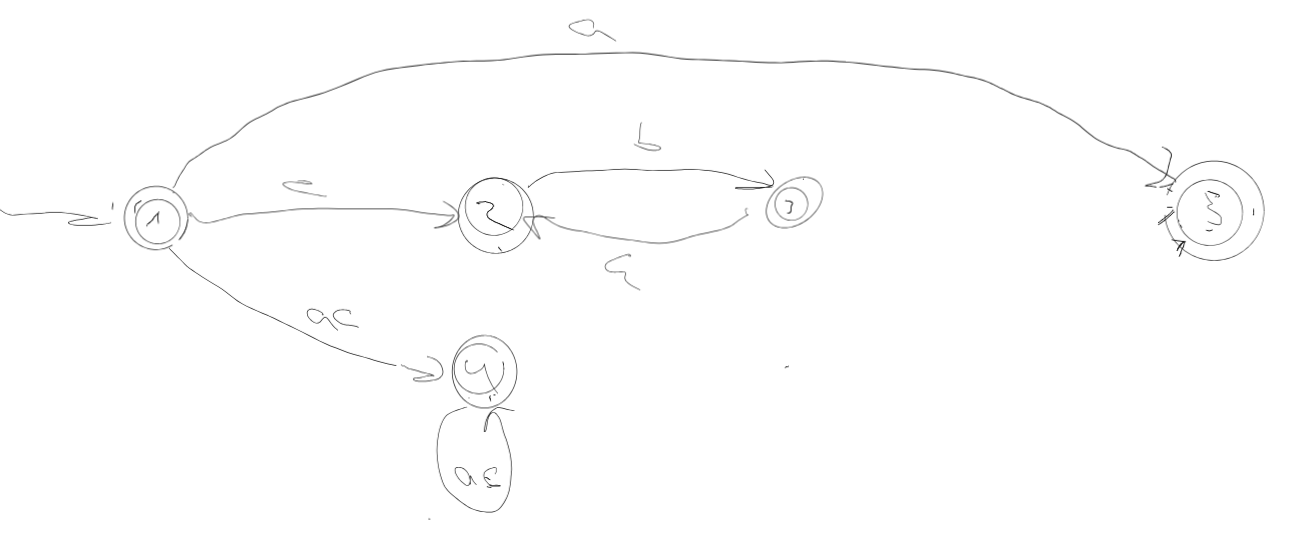
\includegraphics[width=0.6\linewidth]{dea6.png} % use option [width=\linewidth] to change size to linewidth (or 0.6\linewidth for example)

\centering
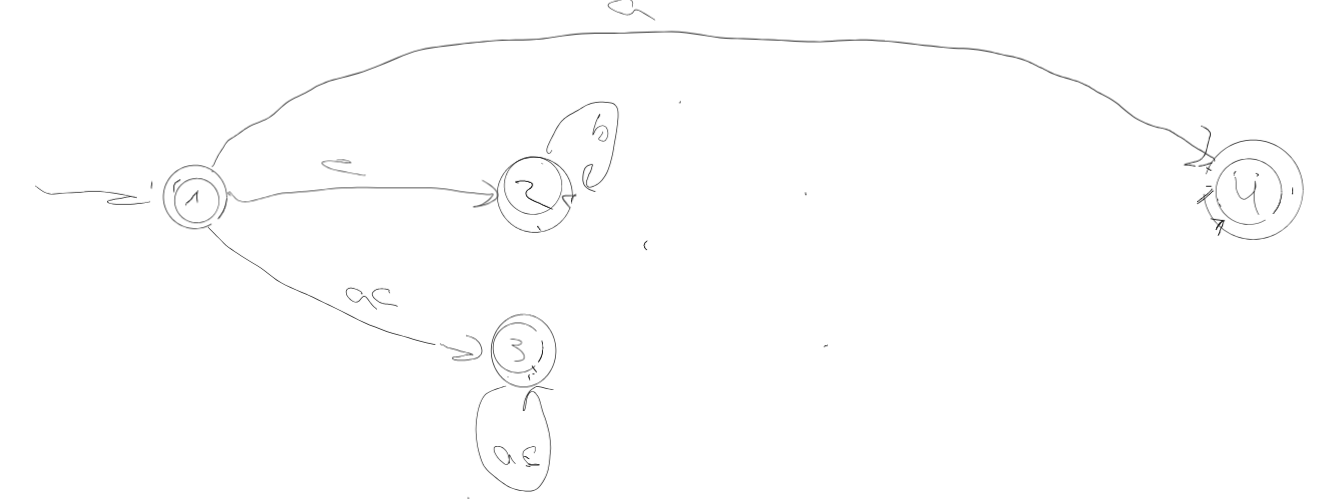
\includegraphics[width=0.6\linewidth]{dea7.png} % use option [width=\linewidth] to change size to linewidth (or 0.6\linewidth for example)

\centering
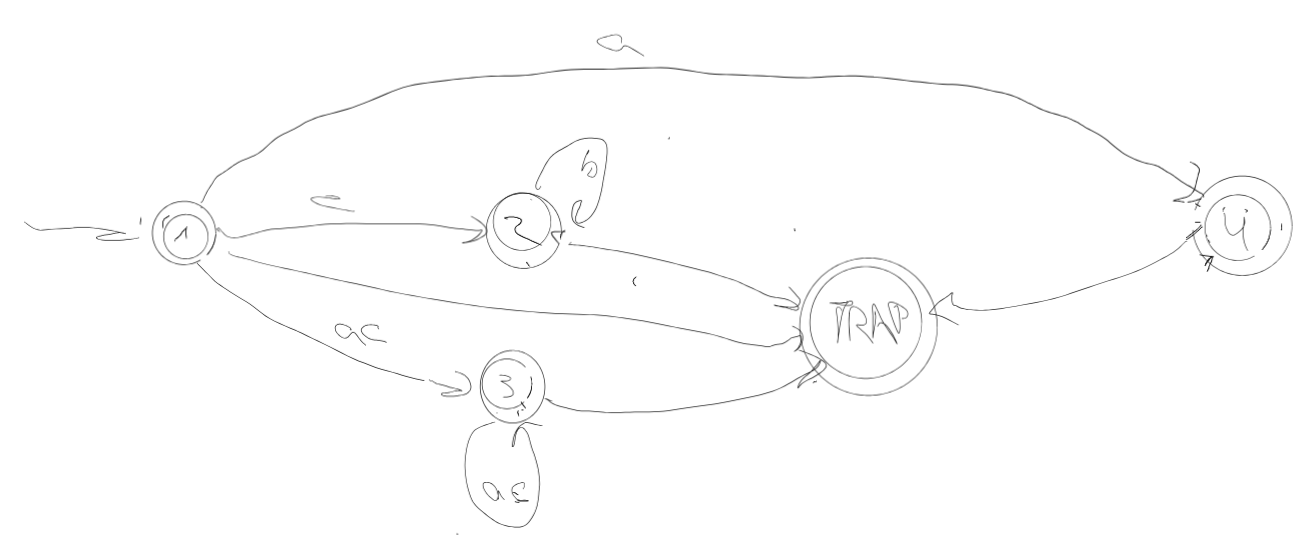
\includegraphics[width=0.6\linewidth]{dea.png} % use option [width=\linewidth] to change size to linewidth (or 0.6\linewidth for example)

Es werden Schrittweise die Epsilon Übergänge entfernt und Zustände zusammengeführt. Im letzten Schritt wird der Fehlerzustand
TRAP hinzugefügt der bei beliebigen nicht definierten Übergängen angesprungen wird. Der Automat ist minimal da keine Äquivalenten
Zustände existieren.

\end{document}